%% ceci est un commentaire 
%% il faut toujours commencer par \documentclass[type de papier, taille de texte]{sytle du document}
\documentclass[a4paper,10pt]{report} %%%% sytle du document : report/book/article


%%%%%%%%%%%%%%%%%%%%%%%%%%%%%%%%%%%%%%%%%%%%%%%%%%%%%%%%%%%%%%%%%%%%%%%%%%%%%%%
%% la suite est une collection des "package" ou des "librararies" pour utiliser des codes spécifiques

%% il vous suffit de les copie-coller quand vous créez un nouveau document TeX (ou bien en ajouter plus si besoin).
\usepackage[utf8]{inputenc} %% pour les accents en français
\usepackage[frenchb]{babel} %% pour un format français
\usepackage{graphicx} %% pour afficher des graphiques
\usepackage{amsmath} %% pour écrire des symboles (maths), des équations, etc.
\usepackage{amssymb}
\usepackage{color}
\usepackage{bm} %% pour lister des citations/la biblio
\usepackage{hyperref} %% pour inserer des liens internet
\usepackage{cleveref} %% pour faire des références uax équations, tableaux, etc.
%\usepackage{setspace} %% pour changer l'espace entre les lignes
%\linespread{1.6} %% pour changer l'espace entre les lignes













%%%%%%%%%%%%%%%%%%%%%%%%%%%%%%%%%%%%%%%%%%%%%%%%%%%%%%%%%%%%%%%%%%%%%%%%%%%%%%%
\title{--------\textbf{Equation de transport}--------} %% choissez un titre approprié à votre sujet
\author{par\\ZHANG Xunjie\\pour le Méthodes numériques pour les EDP M1 } %% utilisez \\ pour une novuelle ligne
\date{fait le 15 mai 2017} %% pour afficher la date actuelle commenter cette ligne














%%%%%%%%%%%%%%%%%%%%%%%%%%%%%%%%%%%%%%%%%%%%%%%%%%%%%%%%%%%%%%%%%%%%%%%%%%%%%%%
%% TOUT ce qui va dans votre rapport doit être entre \begin{document} & \end{document}
\begin{document}
\selectlanguage{french} %% format français
\maketitle %% pour afficher le titre
\tableofcontents %% pour afficher/compiler le sommaire automatiquement
\listoffigures %% pour lister les figures
%%%%%%%%%%%%%%%%%%%%%%%%%%%%%%%%%%%%%%%%%%%%%%






%%%%%%%%%%%%%%%%%%%%%%%%%%%%%%%%%%%%%%%%%%%%%%
\chapter{Problème physique} %% pour commencer un chapitre


Dans cette séance de TP EDP , on considère le problème de l'advection d'une impulsion acoustique; le champ de pression est initialement :
\begin{equation}
    P_0(x)=\left\{
    \begin{array}{r c l}
       &\cos(kx)\exp(-\alpha x^2)\,\,\,\,\,\,\,\,|x|<0.5\\&P_{\infty}\,\,\,\,\,\,\,\,|x|>0.5
    \end{array}
    \right.
\end{equation}


Pour la continuité de la pression initiale et ses dérivées par rapport  à , on met $\alpha=-2k\tan(\frac{k}{2})$ , et $P_{\infty}=\cos(\frac{k}{2})\exp(-\frac{\alpha}{4}$. 

Enfin, pour obtenir une impulsion utile, on utilisera $ k=37$
Pour la propagation on peut utiliser l’équation de transport,
\begin{equation}
\frac{\partial p}{\partial t}+c\frac{\partial p}{\partial x}=0
\end{equation}

Ou  est la pression et est la vitesse du son.
Sur un domaine $-L\leq x\leq 2L$, les conditions au limites sont : 
$p(x=-L)=P_{\infty}$  et  $\frac{\partial p}{\partial x}(x=2L)=0$.

%%%%%%%%%%%%%%%%%%%%%%%%%%%%%%%%%%%%%%%%%%%%%
\chapter{Solution analytique}
La solution générale de ce type de problème avec $c>0$ , s’écrit sous la forme : 
\begin{equation}
p(x,t)=P_0(X) \,\,\,\,\,\,\,\,\,\,\,\,X=x-ct
\end{equation}                       
Alors, 
\begin{equation}
    P_0(x)=\left\{
    \begin{array}{r c l}
       &\cos(kX)\exp(-\alpha X^2)\,\,\,\,\,\,\,\,|x|<0.5\\&P_{\infty}\,\,\,\,\,\,\,\,|x|>0.5
    \end{array}
    \right.
\end{equation}

On considère la propagation d’une onde sonore plane dans tube de longueur 2L contenant un milieu au repos de densité $r_0$ et de pression $p_0$. Le milieu est perturbé à l’instant initial par une fluctuation de pression $\omega(x)$ ne dépendant que de la direction spatiale $x$ et sans vitesse initial $\frac{\partial p}{\partial t}(x,0)=0$. La densité$r(x,t)+r_0$ la pression $p(x,t)+p_0$ et la vitesse $u(x,t)$ du milieu perturbée sont solutions des équations de conservation d’Euler, qui décrivent la dynamique d’un gaz non visqueux. 

En supposant que les perturbations sont faibles (hypothèse de
l’acoustique), l’équation de conservation de la masse s’écrit au premier ordre :
\begin{equation}
\frac{\partial p}{\partial t}+\rho_0\frac{\partial p}{\partial x}=0
\end{equation}
De même l’équation de conservation de la quantité de mouvement s’écrit au premier ordre :
\begin{equation}
\frac{\partial p}{\partial x}+\rho_0\frac{\partial p}{\partial x}=0
\end{equation}

Les fluctuations étant faibles, on peut supposer l’écoulement isentropique :
\begin{equation}
\frac{p}{p_0}=\gamma\frac{\rho}{\rho_0}
\end{equation}

De ces relations on en déduit un système d’équations hyperbolique sur  et  :
\begin{equation}
\frac{\rho_0}{\gamma p_0}\frac{\partial p}{\partial t}+\rho_0\frac{\partial p}{\partial x}=0
\end{equation}
\begin{equation}
p_0\frac{\partial u}{\partial t}+\frac{\partial p}{\partial x}=0
\end{equation}

En dérivant la première équation par rapport à t et la seconde par rapport à x, on obtiens par différence l’équation des ondes pour la fluctuation de pression p :
\begin{equation}
\frac{\partial^2 p}{\partial t^2}+\frac{\gamma p_0}{\rho_0}\frac{\partial p}{\partial x}=0
\end{equation}

%%%%%%%%%%%%%%%%%%%%%%%%%%%%%%%%%%%%%%%%%%%%%%
\chapter{Méthode numérique}

\section{Schéma de courant}

Le schéma s'écrit sous la form suivante :
\begin{equation}
\frac{p^{n+1}_i-p^{n}_i}{\triangle t}= -c\frac{p^{n}_i-p^{n}_{i-1}}{\triangle x}
\end{equation}

On introduce une petite perturpation :
\begin{equation}
p^n_i=p^n_i+\varepsilon^n_i
\end{equation}
en même temps
$$C_{FL}=\frac{c\triangle t}{\triangle x}$$
$$\beta=\omega dx$$
on introduce Fouriere mode :
\begin{equation}
\varepsilon^n_i=\psi ^ne^{I\omega i dx}
\end{equation}
\subsection{Stabilité}
\begin{equation}
\frac{\psi^{n+1}}{\psi^n}=1-C_{FL}(\cos\beta-1)-C_{FL}\sin\beta
\end{equation}
On se trouve la fraction est une valeur complex , donc on cherche la module de cette valeur :
$$\Big|\frac{\psi^{n+1}}{\psi^n}\Big|\leq 1$$
et on retrouve la résultat:
\begin{equation}
\Big|C_{FL}\Big|\leq 1
\end{equation}
\subsection{Consistance }
On utilise Taylor Series pour trouver la consistance :
\begin{equation}
U^{n+1}_i=U^{n}_i+\triangle t \frac{\partial U}{\partial t}\Big|_{(i,n)}+\frac{\triangle t^2}{2} \frac{\partial^2 U}{\partial t^2}\Big|_{(i,n)}+\frac{\triangle t^3}{6} \frac{\partial^3 U}{\partial t^3}\Big|_{(i,n)}+\cdots\cdots
\end{equation}
\\

D'ou ,$U^{n}_i$ est la solution exact .
\\

et on trouve :
\begin{equation}
Err=\frac{\triangle t}{2}\frac{\partial^2 p}{\partial t^2}\Big|_{(i,n)}-\frac{c\triangle x}{2}\frac{\partial^2 p}{\partial x^2}\Big|_{(i,n)}+\circ(\triangle t^2,\triangle x^2)
\end{equation}
\\

Avec :
$$\frac{\partial^2 p}{\partial t^2}=\frac{\partial }{\partial t}\Big(-c\frac{\partial p}{\partial x}\Big)=-c\frac{\partial }{\partial x}\Big(\frac{\partial p}{\partial t}\Big)=-c\frac{\partial }{\partial x}\Big(-c\frac{\partial p}{\partial x}\Big)=c^2\frac{\partial^2 p}{\partial x^2}$$

\begin{equation}
Err=\frac{\triangle tc^2}{2}\frac{\partial^2 p}{\partial x^2}\Big|_{(i,n)}-\frac{c\triangle x}{2}\frac{\partial^2 p}{\partial x^2}\Big|_{(i,n)}+\circ(\triangle t^2,\triangle x^2)
\end{equation}

On a $$C_{FL}=\frac{c\triangle t}{\triangle x}$$ 
\\

Finalement,
\begin{equation}
Err=\frac{c\triangle x}{2}\frac{\partial^2 p}{\partial x^2}\Big(C_{FL}-1\Big)+\circ(\triangle t^2,\triangle x^2)
\end{equation}
\\

On peur dire que il y a une diffusion avec coefficient $\frac{c\triangle x}{2}(C_{FL}-1)$


\section{Schéma de Lax-Wendroff}
Le schéma s'écrit sous la form suivante :
\begin{equation}
\frac{p^{n+1}_i-p^{n}_i}{\triangle t}= -\frac{c}{2\triangle x}\Big(p^{n}_{i+1}-p^{n}_{i-1}\Big)+\frac{c^2\triangle t^2}{2\triangle x^2}\Big(p^{n}_{i+1}-2p^{n}_{i}+p^{n}_{i-1}\Big)
\end{equation}

On introduce une petite perturpation :
\begin{equation}
p^n_i=p^n_i+\varepsilon^n_i
\end{equation}
en même temps
$$C_{FL}=\frac{c\triangle t}{\triangle x}$$
$$\beta=\omega dx$$
on introduce Fouriere mode :
\begin{equation}
\varepsilon^n_i=\psi ^ne^{I\omega i dx}
\end{equation}
\subsection{Stabilité}
\begin{equation}
\frac{\psi^{n+1}}{\psi^n}=1-2C_{FL}^2\sin^2(\frac{\beta}{2})-IC_{FL}(1-\sin\beta)
\end{equation}

On se trouve la fraction est une valeur complex , donc on cherche la module de cette valeur :
$$\Big|\frac{\psi^{n+1}}{\psi^n}\Big|\leq 1$$
et on retrouve la résultat:
\begin{equation}
\Big|C_{FL}\Big|\leq 1
\end{equation}
\subsection{Consistance }
On utilise Taylor Series pour trouver la consistance :
\begin{equation}
U^{n+1}_i=U^{n}_i+\triangle t \frac{\partial U}{\partial t}\Big|_{(i,n)}+\frac{\triangle t^2}{2} \frac{\partial^2 U}{\partial t^2}\Big|_{(i,n)}+\frac{\triangle t^3}{6} \frac{\partial^3 U}{\partial t^3}\Big|_{(i,n)}+\cdots\cdots
\end{equation}
\\

D'ou ,$U^{n}_i$ est la solution exact .
\\

et on a :
$$Err=\frac{p^{n+1}_i-p^{n}_i}{\triangle t}+\frac{c}{2\triangle x}\Big(p^{n}_{i+1}-p^{n}_{i-1}\Big)-\frac{c^2\triangle t^2}{2\triangle x^2}\Big(p^{n}_{i+1}-2p^{n}_{i}+p^{n}_{i-1}\Big)$$

on trouve :
\begin{equation}
Err=\frac{c\triangle x^2}{6}\frac{\partial^3 p}{\partial x^3}\Big|_{(i,n)}+\circ(\triangle t^2,\triangle^4)
\end{equation}
\\

On peur dire que il y a une dispersion avec coefficient $\frac{c\triangle x^2}{6}$

\section{Schéma de leap-frog}

\begin{equation}
\frac{p^{n+1}_i-p^{n-1}_i}{\triangle t}= -c\frac{p^{n}_{i+1}-p^{n}_{i-1}}{\triangle x}
\end{equation}

On introduce une petite perturpation :
\begin{equation}
p^n_i=p^n_i+\varepsilon^n_i
\end{equation}
en même temps
$$C_{FL}=\frac{c\triangle t}{\triangle x}$$
$$\beta=\omega dx$$
on introduce Fouriere mode :
\begin{equation}
\varepsilon^n_i=\psi ^ne^{I\omega i dx}
\end{equation}
\subsection{Stabilité}
On substrust et on trouve :
\begin{equation}
\frac{\psi^{n+1}_{i}}{\psi^{n}_{i}}=\frac{\psi^{n-1}_{i}}{\psi^{n}_{i}}-2IC_{FL}\sin\beta
\end{equation}
Cette valeur de stabilité est une trois-étage ,  on pose :
$$\frac{\psi^{n+1}_{i}}{\psi^{n}_{i}}=\frac{\psi^{n-1}_{i}}{\psi^{n}_{i}}=G$$
on a :
\begin{equation}
G^2+2IC_{FL}\sin\beta-1=0
\end{equation}

Les solutions sont :
$$G_{1,2}=-IC_{FL}\sin\beta\pm(1-C_{FL}^2\sin^2\beta)^{\frac{1}{2}}$$
\\

Ici , on sépare les résultat et discuss :
\begin{itemize}
    \item[$\bullet$]$\triangle\geq 0$  , $G_{1,2}=1$ et on trouve la condition ,$\Big|C_{FL}\Big|\leq 1 $ 
     \item[$\bullet$]$\triangle <0$ , $G_{1,2}=-I(C_{FL}\sin\beta\pm\sqrt{C_{FL}^2\sin^2\beta})$ est une valeur complexe , on essaie cherche la module de cette valeur , 
     $$\Big|G_{1,2}\Big|^2=Im\{G_{1,2}\}^2=(C_{FL}\sin\beta\pm\sqrt{C_{FL}^2\sin^2\beta-1})^2$$
     on s'interest à $G_2$ , et :
     $$G_2^2=(C_{FL}\sin\beta+\sqrt{C_{FL}^2\sin^2\beta-1})^2$$
     $$G_2^2>(C_{FL}\sin\beta)^2>1$$
   on dit que pour $\triangle <0$ , il n'y pas de consisitance .
\end{itemize}

Donc , pour la stabilité de la schéma Leap-Frog , quand $\Big|C_{FL}\Big|\leq 1$ , elle est stabilité avec condition .
\subsection{Consistance }
\begin{equation}
Err=\frac{\triangle t^2}{12}\frac{\partial^3 p}{\partial t^3}\Big|_{(i,n)}+\frac{c\triangle x^2}{12}\frac{\partial^3 p}{\partial x^3}\Big|_{(i,n)}+\circ(\triangle t^4,\triangle x^4)
\end{equation}
On a :
$$\frac{\partial^2 p}{\partial t^2}=\frac{\partial }{\partial t}\Big(-c\frac{\partial p}{\partial x}\Big)=-c\frac{\partial }{\partial x}\Big(\frac{\partial p}{\partial t}\Big)=-c\frac{\partial }{\partial x}\Big(-c\frac{\partial p}{\partial x}\Big)=c^2\frac{\partial^2 p}{\partial x^2}$$
on retrouve :
$$\frac{\partial^3 p}{\partial t^3}=-c^3\frac{\partial^3 p}{\partial x^3}$$
 Donc au final :
 \begin{equation}
 Err=\frac{1}{12}\frac{\partial^3 p}{\partial x^3}\Big|_{(i,n)}(-c^3\triangle t^2+c\triangle x^2)+\circ(\triangle t^4,\triangle x^4)
 \end{equation}
 
 On dit que cette schéma transpose avec dispersion , sa coefficient est $\frac{1}{12}(-c^3\triangle t^2+c\triangle x^2)$.


%%%%%%%%%%%%%%%%%%%%%%%%%%%%%%%%%%%%%%%%%%%%%%
\chapter{Etude numérique}

\section{Solution exact}
\begin{figure}[h]
%% [h] implique que le graphique sera placé ici (et pas en haut ou en bas du document)
\begin{center}
%% pour centré l'image
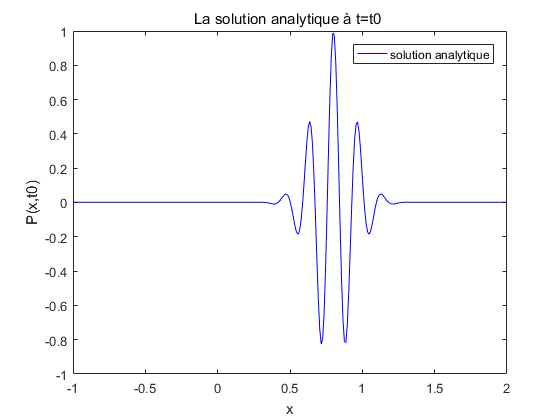
\includegraphics[width=1.0\textwidth]{FIG/figure1.png}
	%% 0.35 fois le largeur du document (\textwidth)
\end{center}
\caption{Solution exact à $t_0$ }
\label{figure1}
\end{figure}

Commentaire :

Au début , on plot cette figure de la solution exact à l'instant $t_0$ . A la vue de la figure , on dit que il est presque vrai , parce-que on trouve l'axe symétrique es$x=0.8$ , c'est la solution transport de la solution $P_0$.


\section{Solution exact et scheme courant}
\begin{figure}[h]
%% [h] implique que le graphique sera placé ici (et pas en haut ou en bas du document)
\begin{center}
%% pour centré l'image
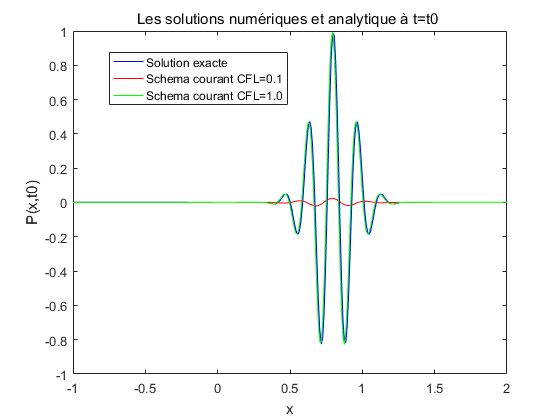
\includegraphics[width=1.0\textwidth]{FIG/figure2.png}
	%% 0.35 fois le largeur du document (\textwidth)
\end{center}
\caption{Solution exact et schéme courant à $t_0$ pour $C_{FL}=0.1\,,1.0$}
\label{figure2}
\end{figure}

Commentaire :
On fait la courant schéma pour different $C_{FL}$ , dans la figure on se trouve , quand $C_{FL}$ égale  1 , la solution exact et la solution numérique sont de chevauchement des deux fonctions . On retrouve la même résultat dans la presentation $Err$ ,$\frac{c\triangle x}{2}(C_{FL}-1)$ est nul , donc les deux solution soit paraille .  Aussi , quand $C_{FL}$ est petite , il y a une grand   diffusion. Et le schéma de Leapfrog a une grande dispersion .

\section{Solution exact et scheme laxwendroff }
\begin{figure}[h]
%% [h] implique que le graphique sera placé ici (et pas en haut ou en bas du document)
\begin{center}
%% pour centré l'image
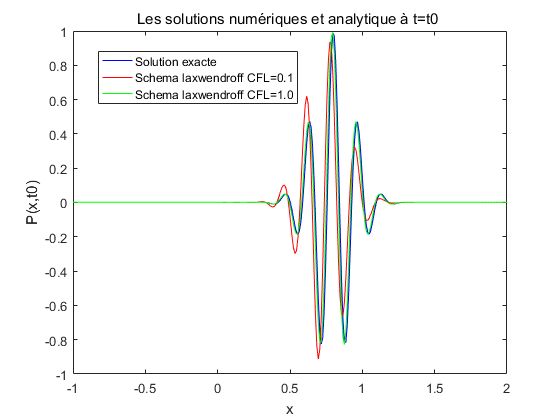
\includegraphics[width=1.0\textwidth]{FIG/figure3.png}
	%% 0.35 fois le largeur du document (\textwidth)
\end{center}
\caption{Solution exact et schéme laxwendroff à $t_0$ pour $C_{FL}=0.1\,,1.0$}
\label{figure3}
\end{figure}
Commentaire:
Dans la figure \ref{figure3} on presente les solution exact et solution de lax wendroff pour 
$C_{FL}=0.1\,,1.0$ , les solution sont similaire que la solution exact . Ils convergent .

\section{Solution exact et scheme leapfrog }
\begin{figure}[h]
%% [h] implique que le graphique sera placé ici (et pas en haut ou en bas du document)
\begin{center}
%% pour centré l'image
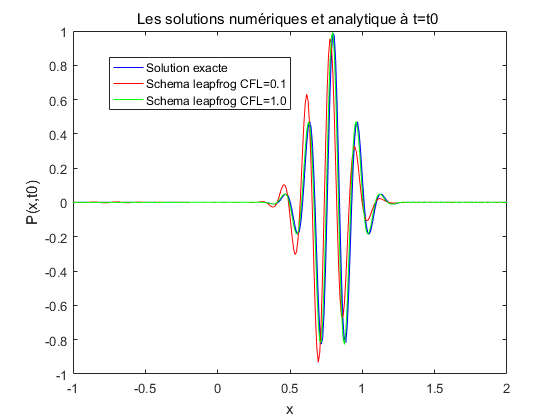
\includegraphics[width=1.0\textwidth]{FIG/figure4.png}
	%% 0.35 fois le largeur du document (\textwidth)
\end{center}
\caption{Solution exact et schéme leapfrog à $t_0$ pour $C_{FL}=0.1\,,1.0$}
\label{figure4}
\end{figure}
Commentaire:
Dans la figure\ref{figure4} on presente les solution exact et solution de la schéma leapfrog  pour 
$C_{FL}=0.1\,,1.0$ , les solution sont similaire que la solution exact . Ils convergent .
\chapter{Erreur numérique}
\section{Error spatial }
\begin{figure}[h]
%% [h] implique que le graphique sera placé ici (et pas en haut ou en bas du document)
\begin{center}
%% pour centré l'image
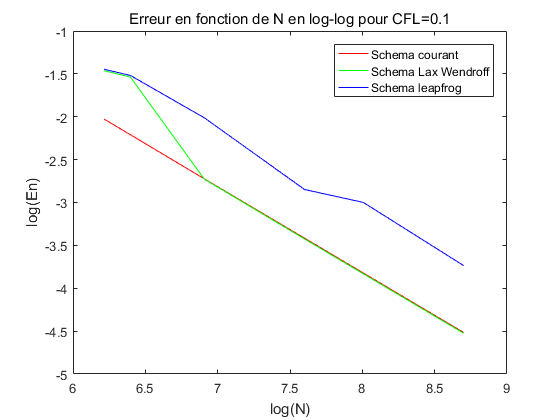
\includegraphics[width=1.0\textwidth]{FIG/figure5.png}
	%% 0.35 fois le largeur du document (\textwidth)
\end{center}
\caption{Error pour les trois schémes }
\label{figure5}
\end{figure}


On va étudier la convergence spatiale de ces trois schémas. On va calculer l’erreur spatiale en fonction de N en utilisant une échelle logarithmique pour les axes, et en déduire la précision spatiale des schémas.
Ici, on prend les discrétisations de N= [500, 600, 1000, 2000, 3000,6000], 
Dans  tous les schémas, on obtient les coefficients  comme le figure au dessus.1, ça veut dire que le schéma de courant est une erreur d’ordre 1 en N. Et les deux autres ont des pentes vers 2.Donc ses erreurs sont d’ordre 2 en N. Dans la code , on peut aussi trouve la pente .


\section{Precision temporelle }
\begin{figure}[h]
%% [h] implique que le graphique sera placé ici (et pas en haut ou en bas du document)
\begin{center}
%% pour centré l'image
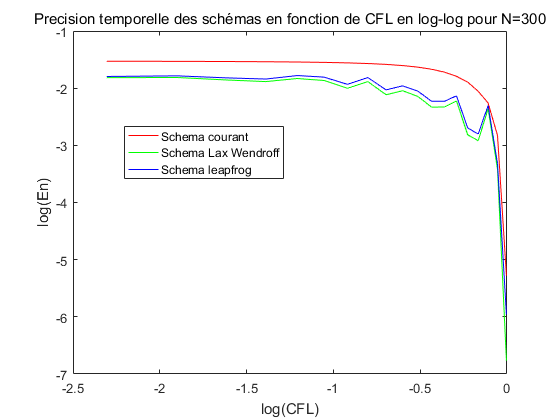
\includegraphics[width=1.0\textwidth]{FIG/figure6.png}
	%% 0.35 fois le largeur du document (\textwidth)
\end{center}
\caption{Precision temporelle pour trois scheme}
\label{figure6}
\end{figure}

On remarque que pour  soit, l’erreur pour ces trois schémas est quasiment constante puisque pour 1, des pas en temps sont inférieurs à des pas en espace, l’erreur est donc contrôlée par la précision spatiale.
 Par contre, pour, soit, les trois schémas sont vérifiés pas par les conditions de stabilité des trois schémas. Les erreurs augmentent très rapidement. Et quand , les erreurs commencer à décroitre. 
 Dans la code , on peut aussi trouve la pente .
%%%%%%%%%%%%%%%%%%%%%%%%%%%%%%%%%%%%%%%%%%%%%%
%%%%%%%%%%%%%%%%%%%%%%%%%%%%%%%%%%%%%%%%%%%%%%
\chapter{Conclusion}

Dans cette séance de TP , on étude équation trensport . Au début on cherche la solution analytique de la problèm  , ensuite on fait une simulation utilisant trois schéma  , schema courant , schéma lax wendroff , et schéma leapfrog . On utilise Matlab pour programmer les solutions .

Pour la schéma courant il y a une diffusion , et pour les autres deux , il y a une dispersion . Les trois schéma sont stabilité avec conditions .   

Pour la précision , on dit que pour la schema courant , la précision est $o(\triangle t^2, \triangle x^2)$ , pour la schema courant , la précision est $o(\triangle t^2, \triangle x^4)$ ,pour la schema courant , la précision est $o(\triangle t^4, \triangle x^4)$ .






\bibliography{MonBiblio.bib}
\bibliographystyle{unsrtnat}	
\end{document}
\grid
